%%%%%%%%%%%%%%%%%%%%%%%%%%%%%%%%%%%%%%%%%
% Bachelor Thesis 
% LaTeX Template
% Version 2.5 (27/8/17)
%
% This template was downloaded from:
% http://www.LaTeXTemplates.com
%
% Version 2.x major modifications by:
% Vel (vel@latextemplates.com)
%
% This template is based on a template by:
% Steve Gunn (http://users.ecs.soton.ac.uk/srg/softwaretools/document/templates/)
% Sunil Patel (http://www.sunilpatel.co.uk/thesis-template/)
%
% Template license:
% CC BY-NC-SA 3.0 (http://creativecommons.org/licenses/by-nc-sa/3.0/)
%\
%%%%%%%%%%%%%%%%%%%%%%%%%%%%%%%%%%%%%%%%%

%----------------------------------------------------------------------------------------
%	PACKAGES AND OTHER DOCUMENT CONFIGURATIONS
%----------------------------------------------------------------------------------------

\documentclass[
11pt, % The default document font size, options: 10pt, 11pt, 12pt
%oneside, % Two side (alternating margins) for binding by default, uncomment to switch to one side
english,
singlespacing, % Single line spacing, alternatives: onehalfspacing or doublespacing
%draft, % Uncomment to enable draft mode (no pictures, no links, overfull hboxes indicated)
%nolistspacing, % If the document is onehalfspacing or doublespacing, uncomment this to set spacing in lists to single
%liststotoc, % Uncomment to add the list of figures/tables/etc to the table of contents
%toctotoc, % Uncomment to add the main table of contents to the table of contents
%parskip, % Uncomment to add space between paragraphs
%nohyperref, % Uncomment to not load the hyperref package
headsepline, % Uncomment to get a line under the header
%chapterinoneline, % Uncomment to place the chapter title next to the number on one line
%consistentlayout, % Uncomment to change the layout of the declaration, abstract and acknowledgements pages to match the default layout
]{BachelorThesis} % The class file specifying the document structure
\usepackage[utf8]{inputenc} % Required for inputting international characters
\usepackage[T1]{fontenc} % Output font encoding for international characters

\usepackage{mathpazo} % Use the Palatino font by default

\usepackage[backend=bibtex,style=authoryear,natbib=true]{biblatex} % Use the bibtex backend with the authoryear citation style (which resembles APA) 

\addbibresource{example.bib} % The filename of the bibliography
\usepackage[autostyle=true]{csquotes} % Required to generate language-dependent quotes in the bibliography

\usepackage{pgfgantt} % in order ot create the Gantt Chart
\usepackage{wrapfig}


%----------------------------------------------------------------------------------------
%	MARGIN SETTINGS
%----------------------------------------------------------------------------------------

\geometry{
	paper=a4paper, % Change to letterpaper for US letter
	inner=2.5cm, % Inner margin
	outer=3.8cm, % Outer margin
	bindingoffset=.5cm, % Binding offset
	top=1.5cm, % Top margin
	bottom=1.5cm, % Bottom margin
	%showframe, % Uncomment to show how the type block is set on the page
}

%----------------------------------------------------------------------------------------
%	THESIS INFORMATION
%----------------------------------------------------------------------------------------

\thesistitle{Comparison of ReactJs and Angular}
\supervisor{Prof. Panagiotis Louridas}
\examiner{} % Your examiner's name, this is not currently used anywhere in the template, print it elsewhere with \examname
\author{Kleio Fragkedaki} % Your name, this is used in the title page and abstract, print it elsewhere with \authorname
\addresses{} % Your address, this is not currently used anywhere in the template, print it elsewhere with \addressname

\keywords{} % Keywords for your thesis, this is not currently used anywhere in the template, print it elsewhere with \keywordnames
\university{\href{https://aueb.gr/}{Athens University of Economics and Business}}
\department{\href{https://my.dmst.aueb.gr/}{Department of Management Science and Technology}} % Your department's name and URL, this is used in the title page and abstract, print it elsewhere with \deptname

\AtBeginDocument{
\hypersetup{pdftitle=\ttitle} % Set the PDF's title to your title
\hypersetup{pdfauthor=\authorname} % Set the PDF's author to your name
\hypersetup{pdfkeywords=\keywordnames} % Set the PDF's keywords to your keywords
}

\makeatletter\@addtoreset{chapter}{part}\makeatother

\begin{document}

\frontmatter % Use roman page numbering style (i, ii, iii, iv...) for the pre-content pages

\pagestyle{plain} % Default to the plain heading style until the thesis style is called for the body content

%----------------------------------------------------------------------------------------
%	TITLE PAGE
%----------------------------------------------------------------------------------------

\begin{titlepage}
\begin{center}

\vspace*{.06\textheight}
{\scshape\LARGE \univname\par}\vspace{1.5cm} % University name
\textsc{\Large Internship Report}\\[0.5cm] % TO DO

\HRule \\[0.4cm] % Horizontal line
{\huge \bfseries \ttitle\par}\vspace{0.4cm} % Thesis title
\HRule \\[1.5cm] % Horizontal line
 
\begin{minipage}[t]{0.4\textwidth}
\begin{flushleft} \large
\emph{Author:}\\
{\authorname} 
\end{flushleft}
\end{minipage}
\begin{minipage}[t]{0.4\textwidth}
\begin{flushright} \large
\emph{Supervisor:} \\
{\supname} 
\end{flushright}
\end{minipage}\\[3cm]
 
\vfill

\large \textit{Internship report and Thesis submitted as part of\\ Bachelor degree}\\[0.3cm]
\textit{in the}\\[0.4cm]
\deptname\\[2cm] % Department name
 
\vfill
\vspace{5cm}

{\large \today}\\[4cm] % Date
%\includegraphics{Logo} % University/department logo - uncomment to place it
 
\end{center}
\end{titlepage}

%----------------------------------------------------------------------------------------
%	LIST OF CONTENTS/FIGURES/TABLES PAGES
%----------------------------------------------------------------------------------------

\tableofcontents % Prints the main table of contents


%----------------------------------------------------------------------------------------
%	ABBREVIATIONS
%----------------------------------------------------------------------------------------

\begin{abbreviations}{ll} % Include a list of abbreviations (a table of two columns)

\textbf{CEO} 		& \textbf{C}hief \textbf{E}xecutive \textbf{O}fficer\\
\textbf{SMT} 		& \textbf{S}enior \textbf{M}anagement \textbf{T}eam\\
\textbf{B2B} 		& \textbf{B}usiness To \textbf{B}usiness\\
\textbf{B2C} 		& \textbf{B}usiness To \textbf{C}ustomer\\
\textbf{CX} 		& \textbf{C}ustomer \textbf{E}xperience\\
\textbf{DOM} 		& \textbf{D}ocument \textbf{O}bject \textbf{M}odel\\
\textbf{HTML}		& \textbf{H}yper \textbf{T}ext \textbf{M}arkup \textbf{L}anguage\\
\textbf{JSON}		& \textbf{J}avaScript \textbf{O}bject \textbf{N}otation\\
\textbf{RPC}        & \textbf{R}emote \textbf{P}rocedure \textbf{C}all \\
\textbf{SPA} 		& \textbf{S}ingle \textbf{P}age \textbf{A}pplication\\
\textbf{UI} 		& \textbf{U}ser \textbf{I}nterface\\
\textbf{URI} 		& \textbf{U}niform \textbf{R}esource \textbf{I}dentifier \\
\textbf{REST} 		& \textbf{R}epresentational \textbf{S}tate \textbf{T}ransfer \\
\textbf{MVC} 		& \textbf{M}odel \textbf{V}iew \textbf{C}ontroller \\
\textbf{Ajax}		& \textbf{A}synchronous \textbf{J}avaScript \textbf{A}nd \textbf{X}ML\\
\textbf{CLI}		& \textbf{C}ommand \textbf{L}ine \textbf{I}nterface \\
\textbf{Framework}	& Reusable software environment to build applications.\\
\textbf{JavaScript} & High-level programming language.\\
\textbf{TypeScript} & Superset of JavaScript which adds optional typing to JavaScript.\\
\textbf{Angular} 	& JavaScript framework maintained by Google.\\
\textbf{React} 		& JavaScript library maintained by Facebook. \\
\textbf{Node.js} 	& Run-time environment for server-side JavaScript.\\
\textbf{NPM}  		& Package manager for Node.js modules. \\

\end{abbreviations}

%----------------------------------------------------------------------------------------
%	THESIS CONTENT - CHAPTERS
%----------------------------------------------------------------------------------------

\mainmatter % Begin numeric (1,2,3...) page numbering

\pagestyle{thesis} % Return the page headers back to the "thesis" style

% Include the chapters of the thesis as separate files from the Chapters folder
% Uncomment the lines as you write the chapters
\part{Internship Report}
% Chapter Template

\chapter{Introduction} % Main chapter title
\label{Chapter1}
As part of my Bachelor degree, I did an internship for three months in Beat, a company that started as a Greek startup about 5 years ago. From March 18th 2019 till June 18th 2019, I contributed as a Software Developer intern in several projects that was referred to a product named "BeatHotels".

\section{Company Description}
%βασικά χαρακτηριστικά κύριες δραστηριότητες

\section{Internship Goal}
 As regards, this internship's goal is gaining experience as a Software Developer, learning tools like React and Redux and understanding how an application works in production mode. Learning how to code in Javascript and improving web site for BeatHotel's agents, and creating npm packages were my main responsibilities as an intern.
 
\section{Report's Structure}
The internship's report is an overview of what I have been interacted with during my internship, analyzing the projects and results, skills that I have gained or used, and my role as an intern in general.

% 5 pages
% Chapter Template

\chapter{Basic Characteristics} % Main chapter title
In the following section I will describe the basic characteristics of my Department’s structure and my role as an intern.
\label{Chapter2} 

\section{ Department }
The Department that I am part of is the Greek Market. Greek Market is managing the marketplace of Greece and is also referred as the Beat of Greece as mentioned in the previous chapter.

\subsection{Role in the Company}
The Greek Market is the only department focused on Greece. Its role inside the company is to manage any demands referred to this marketplace. Demands on marketing, finance, business analysis, customer experience and the development of product BeatHotels that is provided only in Greece, are all responsibility of this department.\par 
The Beat App is developed by other departments and any changes required for the greek marketplace are forwarded from the Greek Market to the Engineering Department of Beat.

\subsection{Department's structure}
Greek Market is constituted by five teams, Operations, Costumer Experience, the Engineer's of Beat Hotels named as GR Squad team, Marketing and Finance team. The General Manager of this Department is Vasilis Danias and the total number of people working in it is 37. 
\begin{figure}[h!]
	\begin{center}
		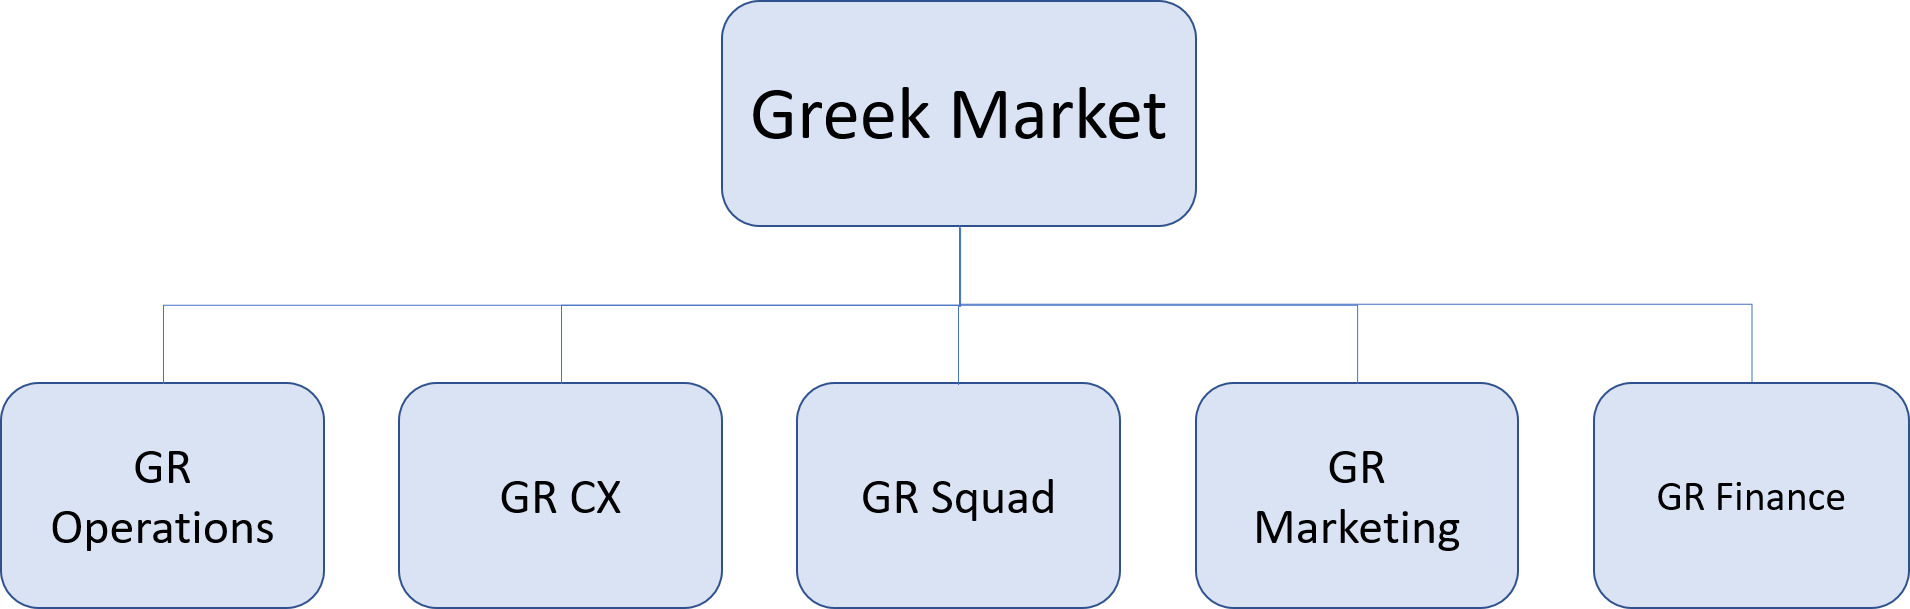
\includegraphics[scale=0.4]{images/GR_Market_structure.png}
	\end{center}
	\caption{Greek Market's structure}
\end{figure}

\subsection{Basic Procedures}
Department's basic procedures are based on the management of three products in the borders of greek market, Hive, Beat App and Beat Hotels.\par
In more details, each team has different responsibilities. CX team is responsible for training drivers, resolving tickets and detecting any problems regarding these three products. The term tickets is any calls or visits made, or emails sent by either a passenger or driver.\par 
Operations team is responsible for designing and controlling the process of production and redesigning business operations in terms of using as few resources as needed and meeting customer requirements. 
Marketing is creating, communicating, delivering, and exchanging offerings that have value for both customers and society in total. Competitions, sponsorships, banners, products or videos created for advertisement and social media management are made by this team.\par
Finance is responsible for beat driver's payments, while GR Squad is the team responsible for developing BeatHotels service.

\subsection{ GR Squad }
GR Squad ia a newly conducted team which is responsible for the development of 
\begin{wrapfigure}[9]{r}{0.3\textwidth}
	\begin{center}
		
\includegraphics[scale=0.25]{images/technologies_used.png}
	\end{center}
	\caption{Technologies Used for BeatHotels}
\end{wrapfigure}
BeatHotel. Team is consisted by eight people, three front-end developers, including myself, three back-end, one Product Owner and one Scrum Master following the agile culture as the other Beat teams.\par 
BeatHotel is a service provided only in Greece and started about seven months ago. The technologies that are used for the development of BeatHotel's driver app, dashboards for each Hotel and Agents' dashboard, are React Native, ReactJS, Node.js and for databases Firebase and Redis.

\section{ My Role }
As a Software Developer Intern in GR Squad team, my role is releasing code that have immediate impact on BeatHotel service's users. \par
At the first one and a half month of my internship, I was a full stack developer and had the opportunity to work on both front and back-end elements of BeatHotel system. During this period, I was responsible to deliver npm packages, code in Node.js and ReactJS in order to complete requested projects for Agent's and Hotels' Dashboards, improve and extend tests and code coverage.\par 
After this period of coding in Javascript for both back and front-end, getting familiar with BeatHotel service, my team and the way things flow, I had to choose between front-end and back-end developer. So, as a front-end I started to deliver tasks only referred to client-side development in order to maintain and extend existing web-site dashboards in ReactJS.
\newpage
\subsection{ Skills Required }
The skills required for this internship are enumerated below.
\begin{itemize}
\item Ability to produce high quality, maintainable and reusable Javascript code in React and Node.js
\item Ability to build a three-layer web application
\item Good knowledge of Unix based Systems
\item Basic understanding of both Sql and N0-Sql databases
\item Ability of problem solving and understanding algorithms complexity
\item Familiar with GitHub Usage
\item Ability to work in a team, communicate ideas, be an active member and deliver on time
\end{itemize}
 
% Chapter Template

\chapter{Projects/Activities} % Main chapter title
%σύντομη περιγραφή όλων των δραστηριοτήτων που ανέλαβα

\label{Chapter3}

During my internship, I participated in quite a few projects that were mostly related to Beat Hotels product, either bugs resolved or entirely new features created, or Greek Marketing’s requirements. All of these projects will be analyzed in this chapter, expect the ones of Chapter \ref{Chapter4} that will just mentioned so as to avoid repetition.

\section{Project 2: Geo - Npm Package}


\begin{figure}[H]
	\begin{center}
		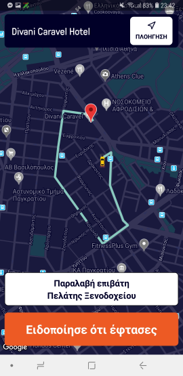
\includegraphics[scale=0.45]{images/my_projects/price_estimator.png}
	\end{center}
	\caption{Approved Pull Request}
\end{figure}

\section{Project 1: Price Estimator- Rides for Approval}

BeatHotel is a totally different product than Beat and a newly introduced one as described in the previous Chapters. For this reason, this new product is combined with a different driver app and a dashboard used by agents, Beat's employees. Agents use the dashboard in order to control rides made through BeatHotel App, start a ride or cancel one if it is needed. This new product does not have any price estimator for the rides made which means that a driver could theoretically add any amount desirable. \par

The project “price estimator” was created for preventing any fraud occurred by drivers. The aim of this project was to estimate the price of a completed ride and compare this price with the actually declared one. In this way, every completed ride is checked  and if it does not pass the validation, it remains as Ride for Approval, so as Agents to check the validate of price gained. \par

This project was the first project ever assigned to me and to one more intern. Our role to this project was to create in Node.js a function for calculating the price of a completed ride based on the data found in database and another function fo validating if the result is approximately equal to the ride's price. We need to mention that every five seconds, each driver sends its location (latitude and longitude), a timestamp (time of the data sent) and other information. So, we used these data gathered in firebase and by using the geo package mentioned earlier and rules of how taxi pricing is in Greece, we managed to get an estimation of the ride. Afterwards, we created one more function for checking the real price with the estimated one. \par

The project lasted about two weeks and it was a great addition to BeatHotel HQ service. We need to clarify that for about a year the service did not have any commissions gained from the driver and that's why it was not a priority at first. Because of this additional feature, Beat's commission is real scenario. \par 

\section{Project 3: Statistics (analyzed in next Chapter)}

"Statistics" project is an external feature in Agent's dashboard that reveals total rides and Gross Merchandise Volume (GMV) gained from BeatHotel service. This project was separated in three main parts, the creation of stats npm package, customized statistics and general statistics, that will be described in detail in next Chapter. Generally, there were added charts in the BeatHotel's web application that present data based on different parameters chosen by Agents. In the chart, the given period's data are also compared with the previous week's or year's data and useful information are extracted for BeatHotel service.

\section{Project 4: Geofence in New Map}
Geofence in New Map- production (feature-deckGLMap)

\section{Project 5: Arc for accepted Drivers in Map}
Arc for accepted Drivers in Map- production (PR)

We want an arc to be added in "Live Map" Tab from the driving vehicle in the map to the pickup location. (12/06/19) (23/05 asana)

\section{Project 6: Babel Configuration for running code in both front-end and back-end}

(13/05/19)

\section{Project 7: Add StartTimestamp- endtimestamp and HQ}
Added to Completed Rides timestamps and link driver to HQ- production (PR)

In "Completed Rides Tab" on Beat Hotels Services - HQ we want to add  the ride ended time named "End Time" in the window which agents see more info about the ride. (6/05/19 asana)

In "Completed Rides Tab" on Beat Hotels Services - HQ we want to add the time of request named "Request Time" of the ride. (requesttimestamp on firebase) in the window which agents see more info about the ride.

In "Completed Rides Tab" on Beat Hotels Services - HQ we want agents by clicking on the Driver's Plates, his profile on HQ ((https://hq-gr.taxibeat.com/driver/edit/9351/) to be appeared.

\section{Project 8: Eliminate Errors in console and eslint errors}
Eliminate Errors in console and eslint errors (PR)

Remove all warnings from console (generated from ESLint) (22/05/19 asana)

\section{Project 9: Add button for unblocking dispatching status-production}
Add button for unblocking dispatching status-production (PR)


\section{Project 10: Landing page for mpaineis-vgaineis (analyzed in next Chapter)}

Landing page for mpaineis-vgaineis is a project referred to the development of a web site for \url{mpaineis-vgaineis.gr} competition of Beat. More specifically, GR Marketing team launched an event in which every week one participant would win a trip abroad. The competition lasted four weeks, and every week there was a different destination. My part to this event was to create the landing page through which every possible user could declare interest in the event, and in this way, to win a trip in one of the destinations. So, I created a responsive to all devices web page, that includes a form for users to declare their interest. The landing page will be online until 7th of June. \par

\section{Project 11: Statistics in Dashboard - "Forecast"}
In Statics in Dashboard Tab, we want in the diagram to be completed for the rest hours of the day that we don't have yet data, from the rides and gmv of the previous week. (18/06)

\section{Project 12: Input location (analyzed in next Chapter)}

BeatHotel is generally a B2B service that aims to fulfill the needs of hotels for a virtual taxi queue. So, the service's dashboards, which is the only way Beat's Agents and Hotels to request for a taxi, used for calling a cub to only one pick-up location, the requested Hotel. However, as the business grows, travel agencies, that were part of the system as well, and some hotels needed to fulfill rides that are having different than Hotel's pick up locations. For this reason, this project occurred and I needed to refactor the Dispatch page, change modal so as to be responsive and add an input for typing any possible different pick-up location. \par

\section{Project 13: Zoom to hotel and driver}

We want when agents are searching for driver plates on "Live Map Tab" to be zoomed in this specific driver. (??)

We want in "Live Map" Tab, to be a filter like "Filter by Plates or Phone" where agents will be able to search a Hotel and the map zooms in the filtered Hotel.

%Θα ήθελα να σας ενημερώσω ότι πλέον μπορείτε στο Live Map, να αναζητήσετε ένα ξενοδοχείο και να κάνει zoom στο αντίστοιχο ξενοδοχείο πάνω στον χάρτη. Να σημειωθεί ότι πρέπει να συμπληρωθεί ακριβώς το ξενοδοχείο που επιθυμείτε εάν πρόκειται για ξενοδοχεία που περιλαμβάνουν την ίδια λέξη. (π.χ. εάν πληκτρολογήσετε την λέξη Divani, δεν θα κάνει zoom σε κάποιο ξενοδοχείο, θα πρέπει να πληκτρολογήσετε Divani Caravel, Divani Apollon, κτλ).

%Zoom in maps: Πλέον στο tab "Live Map", όταν αναζητάτε ένα όχημα βάσει Plates ή Phone, αυτόματα γίνεται zoom, στο οδηγό με αυτά τα στοιχεία. Εδώ να τονιστεί ότι για να γίνει zoom θα πρέπει τα στοιχεία Plates ή Phone να είναι μοναδικά για τον οδηγό εκείνη την στιγμή στον χάρτη. (Εάν δηλαδή μία στιγμή στον χάρτη υπάρχουν δύο οδηγοί που οι πινακίδες τους ξεκινάνε από 13 και πλητρολογήσετε το 13 στο search bar δεν θα γίνει zoom σε κάποιον οδηγό παρά μόνο εάν πληκρολογήσετε ολόκληρη την μοναδική πινακίδα του οδηγού).

\section{Project 14: Restructure Setting Component}

\section{Project 15: Get rid of old maps}

We want to get rid of old maps in completed rides and in approved rides and replace with the new maps. More specifically we have to get rid of the package "React MapboxGL"

%10 pages, 10 projects
% Chapter Template

\chapter{Results} % Main chapter title
%choose two or three projects, check report

\label{Chapter4}

\section{Project 1}

\subsection{Description}

\subsection{Best Practices}

\subsection{Schedule}

\subsection{Problems occurred}

\section{Project 2}

\subsection{Description}

\subsection{Best Practices}

\subsection{Schedule}

\subsection{Problems occurred}

%6 pages 2 per projects
 
% Chapter Template

\chapter{Updated Time Management} % Main chapter title
\label{Chapter5}

\section{Time Schedule}
\begin{center}
	\begin{tabular}{ |p{7cm}|p{3cm}|  }
		\hline
		\textbf{Activity} & \textbf{Duration} \\ [0.3cm]
		\hline
		 Getting to know BeatHotel's system, Node.js and React.js 
		 											&  18/03- 26/03 \\[0.4cm]
		\hline
		Price Estimator Development in Node.js \& Creation of Geo package 
													&  27/03- 10/04  \\[0.4cm]
		\hline
		Both General and Customized Statistics Development in ReactJS \& Creation of Stats package
													&  11/04- 25/04  \\[0.4cm]
		\hline
		Geofence and Arc Added to BeatHotel's map displayed in agent's dashboard 
													&  29/04- 30/04  \\[0.4cm]
		\hline
		Bugs and Fixes occurred in BeatHotel HQ dashboard
													&  23/04- 9/05  \\[0.4cm]
		\hline
		Add button for unblocking dispatching status-production
													&  13/05- 15/05  \\[0.4cm]
		\hline
		Landing page of mpaineis-vgaineis competition 
													&  16/05- 24/05  \\[0.4cm]
		\hline
		Feature Input Pick up Location 
													&  27/03- 30/05  \\[0.4cm]
		\hline
		Feature for zooming to Hotel and to Driver 		
													&  3/06- 5/06  	\\[0.4cm]
		\hline
		Replace old maps						    &  6/06 and 10/06 \\[0.4cm]
		\hline
		Restructure of Setting Component			&  11/06- 13/06  \\[0.4cm]
		\hline
		Restructuring and upgrading the whole project   
													&  18/06- ongoing  \\[0.4cm]
		\hline
	\end{tabular}
\end{center}

\section{Gantt Chart}
\begin{ganttchart}{1}{14}
	\gantttitle{Gant Chart}{14} \\
	\gantttitlelist{1,...,14}{1} \\
	\ganttbar{Getting to know the system}{1}{2} \ganttnewline
	\ganttlinkedbar{Price Estimator}{3}{4} \ganttnewline
	\ganttlinkedbar{Statistics}{5}{7} \ganttnewline
	\ganttmilestone{Statistics \& Price Estimator Online}{7} \ganttnewline
	\ganttlinkedbar{Features and Fixes on BeatHotels}{7}{9} \ganttnewline
	\ganttlinkedbar{Mpaineis-Vgaineis}{10}{11} \ganttnewline
	\ganttmilestone{Mpaineis-Vgaineis Live}{12} \ganttnewline
	\ganttlinkedbar{Feature Input Pick up Location}{12}{12} \ganttnewline
	\ganttlinkedbar{Zoom to Hotel/Driver \& new Maps}{13}{13} \ganttnewline
	\ganttbar{Restructure Components}{12}{14}
	\ganttlink{elem2}{elem3}
	\ganttlink{elem3}{elem4}
	\ganttlink{elem4}{elem5}
	\ganttlink{elem5}{elem6}
	\ganttlink{elem6}{elem7}
	\ganttlink{elem7}{elem8}
	\ganttlink{elem8}{elem9}
\end{ganttchart} 
% Chapter Template

\chapter{Conclusion} % Main chapter title
\label{Chapter5} % Change 5 to a consecutive number; for referencing this chapter elsewhere, use \ref{Chapter5}

During this thesis, there were analyzed both fundamental concepts of web applications, including the different architectural approaches and historical references, and the two most popular front-end tools for building web projects, React and AngularJS. The main purpose was to compare ReactJS and Angular, a frequently defined question among newcomer companies and developers. This comparison took place based on different metrics that cite each framework/library's advantages and disadvantages.

\section{Future Work}
To complete ReactJS and Angular's comparison in all possible perspectives, performance needs to examined and proven. In future work, creating the same application in both client-side tools can provide an equal and more objective correlation. In this sense, I aim to build my app, Hom-e, which is developed in Angular, in React as well and then check the performance and user experience of both apps.


\addtocontents{toc}{\protect\newpage}

\part{Thesis}
% Chapter Template

\chapter{Introduction} % Main chapter title
\label{Chapter1}
As part of my Bachelor degree, I did an internship for three months in Beat, a company that started as a Greek startup about 5 years ago. From March 18th 2019 till June 18th 2019, I contributed as a Software Developer intern in several projects that was referred to a product named "BeatHotels".

\section{Company Description}
%βασικά χαρακτηριστικά κύριες δραστηριότητες

\section{Internship Goal}
 As regards, this internship's goal is gaining experience as a Software Developer, learning tools like React and Redux and understanding how an application works in production mode. Learning how to code in Javascript and improving web site for BeatHotel's agents, and creating npm packages were my main responsibilities as an intern.
 
\section{Report's Structure}
The internship's report is an overview of what I have been interacted with during my internship, analyzing the projects and results, skills that I have gained or used, and my role as an intern in general.

% 5 pages
% Chapter Template

\chapter{Basic Characteristics} % Main chapter title
In the following section I will describe the basic characteristics of my Department’s structure and my role as an intern.
\label{Chapter2} 

\section{ Department }
The Department that I am part of is the Greek Market. Greek Market is managing the marketplace of Greece and is also referred as the Beat of Greece as mentioned in the previous chapter.

\subsection{Role in the Company}
The Greek Market is the only department focused on Greece. Its role inside the company is to manage any demands referred to this marketplace. Demands on marketing, finance, business analysis, customer experience and the development of product BeatHotels that is provided only in Greece, are all responsibility of this department.\par 
The Beat App is developed by other departments and any changes required for the greek marketplace are forwarded from the Greek Market to the Engineering Department of Beat.

\subsection{Department's structure}
Greek Market is constituted by five teams, Operations, Costumer Experience, the Engineer's of Beat Hotels named as GR Squad team, Marketing and Finance team. The General Manager of this Department is Vasilis Danias and the total number of people working in it is 37. 
\begin{figure}[h!]
	\begin{center}
		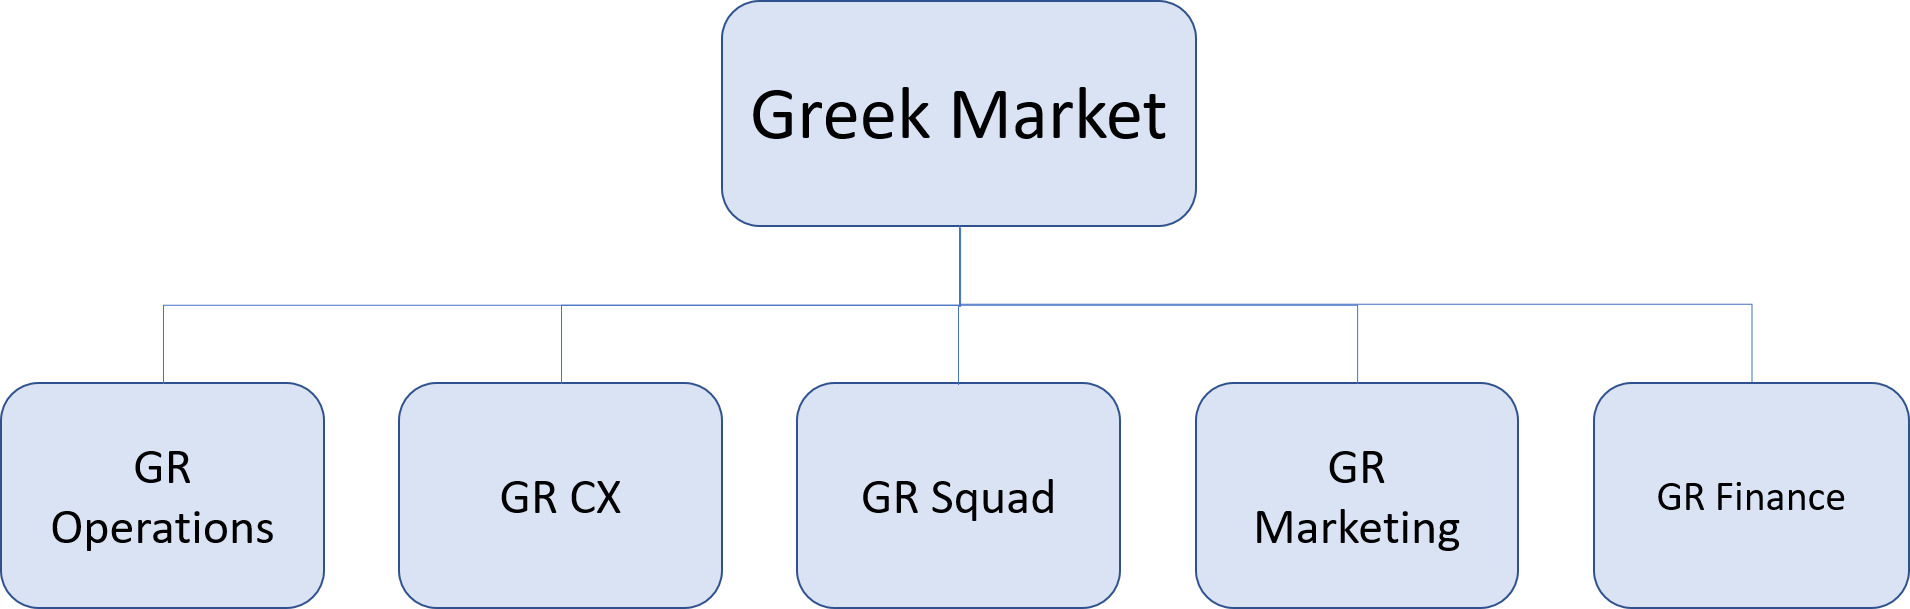
\includegraphics[scale=0.4]{images/GR_Market_structure.png}
	\end{center}
	\caption{Greek Market's structure}
\end{figure}

\subsection{Basic Procedures}
Department's basic procedures are based on the management of three products in the borders of greek market, Hive, Beat App and Beat Hotels.\par
In more details, each team has different responsibilities. CX team is responsible for training drivers, resolving tickets and detecting any problems regarding these three products. The term tickets is any calls or visits made, or emails sent by either a passenger or driver.\par 
Operations team is responsible for designing and controlling the process of production and redesigning business operations in terms of using as few resources as needed and meeting customer requirements. 
Marketing is creating, communicating, delivering, and exchanging offerings that have value for both customers and society in total. Competitions, sponsorships, banners, products or videos created for advertisement and social media management are made by this team.\par
Finance is responsible for beat driver's payments, while GR Squad is the team responsible for developing BeatHotels service.

\subsection{ GR Squad }
GR Squad ia a newly conducted team which is responsible for the development of 
\begin{wrapfigure}[9]{r}{0.3\textwidth}
	\begin{center}
		
\includegraphics[scale=0.25]{images/technologies_used.png}
	\end{center}
	\caption{Technologies Used for BeatHotels}
\end{wrapfigure}
BeatHotel. Team is consisted by eight people, three front-end developers, including myself, three back-end, one Product Owner and one Scrum Master following the agile culture as the other Beat teams.\par 
BeatHotel is a service provided only in Greece and started about seven months ago. The technologies that are used for the development of BeatHotel's driver app, dashboards for each Hotel and Agents' dashboard, are React Native, ReactJS, Node.js and for databases Firebase and Redis.

\section{ My Role }
As a Software Developer Intern in GR Squad team, my role is releasing code that have immediate impact on BeatHotel service's users. \par
At the first one and a half month of my internship, I was a full stack developer and had the opportunity to work on both front and back-end elements of BeatHotel system. During this period, I was responsible to deliver npm packages, code in Node.js and ReactJS in order to complete requested projects for Agent's and Hotels' Dashboards, improve and extend tests and code coverage.\par 
After this period of coding in Javascript for both back and front-end, getting familiar with BeatHotel service, my team and the way things flow, I had to choose between front-end and back-end developer. So, as a front-end I started to deliver tasks only referred to client-side development in order to maintain and extend existing web-site dashboards in ReactJS.
\newpage
\subsection{ Skills Required }
The skills required for this internship are enumerated below.
\begin{itemize}
\item Ability to produce high quality, maintainable and reusable Javascript code in React and Node.js
\item Ability to build a three-layer web application
\item Good knowledge of Unix based Systems
\item Basic understanding of both Sql and N0-Sql databases
\item Ability of problem solving and understanding algorithms complexity
\item Familiar with GitHub Usage
\item Ability to work in a team, communicate ideas, be an active member and deliver on time
\end{itemize}
 
% Chapter Template

\chapter{Projects/Activities} % Main chapter title
%σύντομη περιγραφή όλων των δραστηριοτήτων που ανέλαβα

\label{Chapter3}

During my internship, I participated in quite a few projects that were mostly related to Beat Hotels product, either bugs resolved or entirely new features created, or Greek Marketing’s requirements. All of these projects will be analyzed in this chapter, expect the ones of Chapter \ref{Chapter4} that will just mentioned so as to avoid repetition.

\section{Project 2: Geo - Npm Package}


\begin{figure}[H]
	\begin{center}
		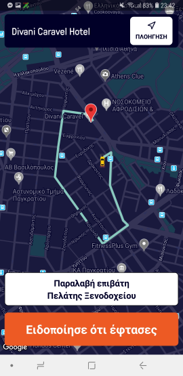
\includegraphics[scale=0.45]{images/my_projects/price_estimator.png}
	\end{center}
	\caption{Approved Pull Request}
\end{figure}

\section{Project 1: Price Estimator- Rides for Approval}

BeatHotel is a totally different product than Beat and a newly introduced one as described in the previous Chapters. For this reason, this new product is combined with a different driver app and a dashboard used by agents, Beat's employees. Agents use the dashboard in order to control rides made through BeatHotel App, start a ride or cancel one if it is needed. This new product does not have any price estimator for the rides made which means that a driver could theoretically add any amount desirable. \par

The project “price estimator” was created for preventing any fraud occurred by drivers. The aim of this project was to estimate the price of a completed ride and compare this price with the actually declared one. In this way, every completed ride is checked  and if it does not pass the validation, it remains as Ride for Approval, so as Agents to check the validate of price gained. \par

This project was the first project ever assigned to me and to one more intern. Our role to this project was to create in Node.js a function for calculating the price of a completed ride based on the data found in database and another function fo validating if the result is approximately equal to the ride's price. We need to mention that every five seconds, each driver sends its location (latitude and longitude), a timestamp (time of the data sent) and other information. So, we used these data gathered in firebase and by using the geo package mentioned earlier and rules of how taxi pricing is in Greece, we managed to get an estimation of the ride. Afterwards, we created one more function for checking the real price with the estimated one. \par

The project lasted about two weeks and it was a great addition to BeatHotel HQ service. We need to clarify that for about a year the service did not have any commissions gained from the driver and that's why it was not a priority at first. Because of this additional feature, Beat's commission is real scenario. \par 

\section{Project 3: Statistics (analyzed in next Chapter)}

"Statistics" project is an external feature in Agent's dashboard that reveals total rides and Gross Merchandise Volume (GMV) gained from BeatHotel service. This project was separated in three main parts, the creation of stats npm package, customized statistics and general statistics, that will be described in detail in next Chapter. Generally, there were added charts in the BeatHotel's web application that present data based on different parameters chosen by Agents. In the chart, the given period's data are also compared with the previous week's or year's data and useful information are extracted for BeatHotel service.

\section{Project 4: Geofence in New Map}
Geofence in New Map- production (feature-deckGLMap)

\section{Project 5: Arc for accepted Drivers in Map}
Arc for accepted Drivers in Map- production (PR)

We want an arc to be added in "Live Map" Tab from the driving vehicle in the map to the pickup location. (12/06/19) (23/05 asana)

\section{Project 6: Babel Configuration for running code in both front-end and back-end}

(13/05/19)

\section{Project 7: Add StartTimestamp- endtimestamp and HQ}
Added to Completed Rides timestamps and link driver to HQ- production (PR)

In "Completed Rides Tab" on Beat Hotels Services - HQ we want to add  the ride ended time named "End Time" in the window which agents see more info about the ride. (6/05/19 asana)

In "Completed Rides Tab" on Beat Hotels Services - HQ we want to add the time of request named "Request Time" of the ride. (requesttimestamp on firebase) in the window which agents see more info about the ride.

In "Completed Rides Tab" on Beat Hotels Services - HQ we want agents by clicking on the Driver's Plates, his profile on HQ ((https://hq-gr.taxibeat.com/driver/edit/9351/) to be appeared.

\section{Project 8: Eliminate Errors in console and eslint errors}
Eliminate Errors in console and eslint errors (PR)

Remove all warnings from console (generated from ESLint) (22/05/19 asana)

\section{Project 9: Add button for unblocking dispatching status-production}
Add button for unblocking dispatching status-production (PR)


\section{Project 10: Landing page for mpaineis-vgaineis (analyzed in next Chapter)}

Landing page for mpaineis-vgaineis is a project referred to the development of a web site for \url{mpaineis-vgaineis.gr} competition of Beat. More specifically, GR Marketing team launched an event in which every week one participant would win a trip abroad. The competition lasted four weeks, and every week there was a different destination. My part to this event was to create the landing page through which every possible user could declare interest in the event, and in this way, to win a trip in one of the destinations. So, I created a responsive to all devices web page, that includes a form for users to declare their interest. The landing page will be online until 7th of June. \par

\section{Project 11: Statistics in Dashboard - "Forecast"}
In Statics in Dashboard Tab, we want in the diagram to be completed for the rest hours of the day that we don't have yet data, from the rides and gmv of the previous week. (18/06)

\section{Project 12: Input location (analyzed in next Chapter)}

BeatHotel is generally a B2B service that aims to fulfill the needs of hotels for a virtual taxi queue. So, the service's dashboards, which is the only way Beat's Agents and Hotels to request for a taxi, used for calling a cub to only one pick-up location, the requested Hotel. However, as the business grows, travel agencies, that were part of the system as well, and some hotels needed to fulfill rides that are having different than Hotel's pick up locations. For this reason, this project occurred and I needed to refactor the Dispatch page, change modal so as to be responsive and add an input for typing any possible different pick-up location. \par

\section{Project 13: Zoom to hotel and driver}

We want when agents are searching for driver plates on "Live Map Tab" to be zoomed in this specific driver. (??)

We want in "Live Map" Tab, to be a filter like "Filter by Plates or Phone" where agents will be able to search a Hotel and the map zooms in the filtered Hotel.

%Θα ήθελα να σας ενημερώσω ότι πλέον μπορείτε στο Live Map, να αναζητήσετε ένα ξενοδοχείο και να κάνει zoom στο αντίστοιχο ξενοδοχείο πάνω στον χάρτη. Να σημειωθεί ότι πρέπει να συμπληρωθεί ακριβώς το ξενοδοχείο που επιθυμείτε εάν πρόκειται για ξενοδοχεία που περιλαμβάνουν την ίδια λέξη. (π.χ. εάν πληκτρολογήσετε την λέξη Divani, δεν θα κάνει zoom σε κάποιο ξενοδοχείο, θα πρέπει να πληκτρολογήσετε Divani Caravel, Divani Apollon, κτλ).

%Zoom in maps: Πλέον στο tab "Live Map", όταν αναζητάτε ένα όχημα βάσει Plates ή Phone, αυτόματα γίνεται zoom, στο οδηγό με αυτά τα στοιχεία. Εδώ να τονιστεί ότι για να γίνει zoom θα πρέπει τα στοιχεία Plates ή Phone να είναι μοναδικά για τον οδηγό εκείνη την στιγμή στον χάρτη. (Εάν δηλαδή μία στιγμή στον χάρτη υπάρχουν δύο οδηγοί που οι πινακίδες τους ξεκινάνε από 13 και πλητρολογήσετε το 13 στο search bar δεν θα γίνει zoom σε κάποιον οδηγό παρά μόνο εάν πληκρολογήσετε ολόκληρη την μοναδική πινακίδα του οδηγού).

\section{Project 14: Restructure Setting Component}

\section{Project 15: Get rid of old maps}

We want to get rid of old maps in completed rides and in approved rides and replace with the new maps. More specifically we have to get rid of the package "React MapboxGL"

%10 pages, 10 projects
% Chapter Template

\chapter{Results} % Main chapter title
%choose two or three projects, check report

\label{Chapter4}

\section{Project 1}

\subsection{Description}

\subsection{Best Practices}

\subsection{Schedule}

\subsection{Problems occurred}

\section{Project 2}

\subsection{Description}

\subsection{Best Practices}

\subsection{Schedule}

\subsection{Problems occurred}

%6 pages 2 per projects
 
% Chapter Template

\chapter{Updated Time Management} % Main chapter title
\label{Chapter5}

\section{Time Schedule}
\begin{center}
	\begin{tabular}{ |p{7cm}|p{3cm}|  }
		\hline
		\textbf{Activity} & \textbf{Duration} \\ [0.3cm]
		\hline
		 Getting to know BeatHotel's system, Node.js and React.js 
		 											&  18/03- 26/03 \\[0.4cm]
		\hline
		Price Estimator Development in Node.js \& Creation of Geo package 
													&  27/03- 10/04  \\[0.4cm]
		\hline
		Both General and Customized Statistics Development in ReactJS \& Creation of Stats package
													&  11/04- 25/04  \\[0.4cm]
		\hline
		Geofence and Arc Added to BeatHotel's map displayed in agent's dashboard 
													&  29/04- 30/04  \\[0.4cm]
		\hline
		Bugs and Fixes occurred in BeatHotel HQ dashboard
													&  23/04- 9/05  \\[0.4cm]
		\hline
		Add button for unblocking dispatching status-production
													&  13/05- 15/05  \\[0.4cm]
		\hline
		Landing page of mpaineis-vgaineis competition 
													&  16/05- 24/05  \\[0.4cm]
		\hline
		Feature Input Pick up Location 
													&  27/03- 30/05  \\[0.4cm]
		\hline
		Feature for zooming to Hotel and to Driver 		
													&  3/06- 5/06  	\\[0.4cm]
		\hline
		Replace old maps						    &  6/06 and 10/06 \\[0.4cm]
		\hline
		Restructure of Setting Component			&  11/06- 13/06  \\[0.4cm]
		\hline
		Restructuring and upgrading the whole project   
													&  18/06- ongoing  \\[0.4cm]
		\hline
	\end{tabular}
\end{center}

\section{Gantt Chart}
\begin{ganttchart}{1}{14}
	\gantttitle{Gant Chart}{14} \\
	\gantttitlelist{1,...,14}{1} \\
	\ganttbar{Getting to know the system}{1}{2} \ganttnewline
	\ganttlinkedbar{Price Estimator}{3}{4} \ganttnewline
	\ganttlinkedbar{Statistics}{5}{7} \ganttnewline
	\ganttmilestone{Statistics \& Price Estimator Online}{7} \ganttnewline
	\ganttlinkedbar{Features and Fixes on BeatHotels}{7}{9} \ganttnewline
	\ganttlinkedbar{Mpaineis-Vgaineis}{10}{11} \ganttnewline
	\ganttmilestone{Mpaineis-Vgaineis Live}{12} \ganttnewline
	\ganttlinkedbar{Feature Input Pick up Location}{12}{12} \ganttnewline
	\ganttlinkedbar{Zoom to Hotel/Driver \& new Maps}{13}{13} \ganttnewline
	\ganttbar{Restructure Components}{12}{14}
	\ganttlink{elem2}{elem3}
	\ganttlink{elem3}{elem4}
	\ganttlink{elem4}{elem5}
	\ganttlink{elem5}{elem6}
	\ganttlink{elem6}{elem7}
	\ganttlink{elem7}{elem8}
	\ganttlink{elem8}{elem9}
\end{ganttchart} 
% Chapter Template

\chapter{Conclusion} % Main chapter title
\label{Chapter5} % Change 5 to a consecutive number; for referencing this chapter elsewhere, use \ref{Chapter5}

During this thesis, there were analyzed both fundamental concepts of web applications, including the different architectural approaches and historical references, and the two most popular front-end tools for building web projects, React and AngularJS. The main purpose was to compare ReactJS and Angular, a frequently defined question among newcomer companies and developers. This comparison took place based on different metrics that cite each framework/library's advantages and disadvantages.

\section{Future Work}
To complete ReactJS and Angular's comparison in all possible perspectives, performance needs to examined and proven. In future work, creating the same application in both client-side tools can provide an equal and more objective correlation. In this sense, I aim to build my app, Hom-e, which is developed in Angular, in React as well and then check the performance and user experience of both apps.



%----------------------------------------------------------------------------------------
%	BIBLIOGRAPHY
%----------------------------------------------------------------------------------------

\printbibliography[title={References}]

%----------------------------------------------------------------------------------------

\end{document}  
